\documentclass{article}

\usepackage{graphicx} % Graphics package
\usepackage[affil-it]{authblk} % Nice author formatting

\usepackage{float} % For figures
\usepackage{subfigure} % For subfigures
\usepackage[labelfont=bf, center]{caption} % Bolds figure titles
\renewcommand{\figurename}{Fig.} % Renames 'Figure' to 'Fig.' when called
\captionsetup{labelsep = period} % Changes : to . for captions

\usepackage{multicol} % For multi-column lists
\usepackage{verbatim} % For block commenting.

\usepackage{listings} % For code blocks.
\lstset{ % Style for code blocks.
	basicstyle=\ttfamily,
	breaklines=true,
	frame=single,
	language=Python,
	tabsize=2,
}

\usepackage{tikz} % For 2D diagrams
\usetikzlibrary{arrows,shapes,trees,shapes.geometric,positioning} % Tikz library extensions
\usepackage{rotating} % For rotate box: used here for rotating figures but keeping labels untouched


\title{UPennalizers \\Robocup 2014 Standard Platform League \\Team Description Paper}
\author{Christopher Akatsuka, Yizheng He, Jianqiao Li,\\ Tatenda Mushonga, Sagar Poudel, Junda Zhu, and\\Dr. Daniel Lee}
\affil{General Robotics Automation, Sensing and Perception (GRASP) Laboratory \\University of Pennsylvania}
\date{} %Exclude date.

\begin{document}

\maketitle

\begin{abstract}
 	This paper presents the organization and architecture of a team of soccer-playing Nao robots developed by University of Pennsylvania's Robocup SPL team. It also documents the efforts gone into improving the code base for the 2014 competitive season. All sensory and motor functions are prototyped and run in Lua on the embedded on board processors. High-level behaviors and team coordination modules are implemented by Lua using state machines. The locomotion engine allows for omni-directional motions and uses sensory feedback to compensate for external disturbances. The cognition module helps robot to detect landmarks and localize in a symmetric environment. Through the year, improvements were made across all of the various modules. 
\end{abstract}

\pagebreak
%\tableofcontents



\section{Introduction}
	In 1999, two years after the first international Robocup meet, the University of Pennsylvania formed the UPennalizers autonomous robot soccer group and began stepping up to the challenges put forth by the competition. While the league was still utilizing four-legged Sony Aibos, the UPennalizers made the quarterfinal rounds every year through 2006 before taking a brief two-year hiatus in 2007. The team reformed and returned in 2009 to begin competing in the Standard Platform League with Aldebaran Naos, taking on bipedal motion alongside improved vision techniques and advanced team behaviors. 

	Continuing its streak of making the international quarterfinals through 2012, the UPennalizers were challenged in 2013 with training a team of entirely new undergraduates without its seasoned veterans from previous years. In 2014, with existing veterans and more talents joining, the team modified the locomotion engine and rebuilt the cognition module. It went on to take first place at the 2014 US Open, and made it to the knock-out phase of Robocup 2014 in Brazil, ranking 9 of 20.



\section{Software Architecture}
	A high-level description of the software architecture for the Naos is shown in Figure \ref{fig:softarch}. The current architecture is an expansion upon the previous years work. It uses Lua as a common development platform to interface between all modules.

	The system maintains a constant update speed of 100Hz, and is decoupled into two separate pipelines. The main process handles motion control and behavior control, while an auxiliary process is dedicated solely to cognition processing. This decision allows for more efficient handling of the Nao's on-board single-core Intel Atom Z530 clocked at 1.6 GHz. The cognition engine runs off of the remaining processing power not used by the main modules, and as a result, the Naos were noted to be much more stable and robust than in previous years.

	Low-level interactions with hardware are implemented using compiled C libraries in conjunction with the Nao's on-board hardware controller (NaoQi) or custom controllers. These in turn, are called via Lua scripts, and allow for control over motor positions, motor stiffnesses, and LED's. Sensory feedback is also handled similarly, allowing users to get data from a variety of sources such as the Nao's two on-board cameras, foot weight sensors, the inertial measurement unit (IMU), and the ultrasound microphones.

	\begin{figure}[H]
		\centering
		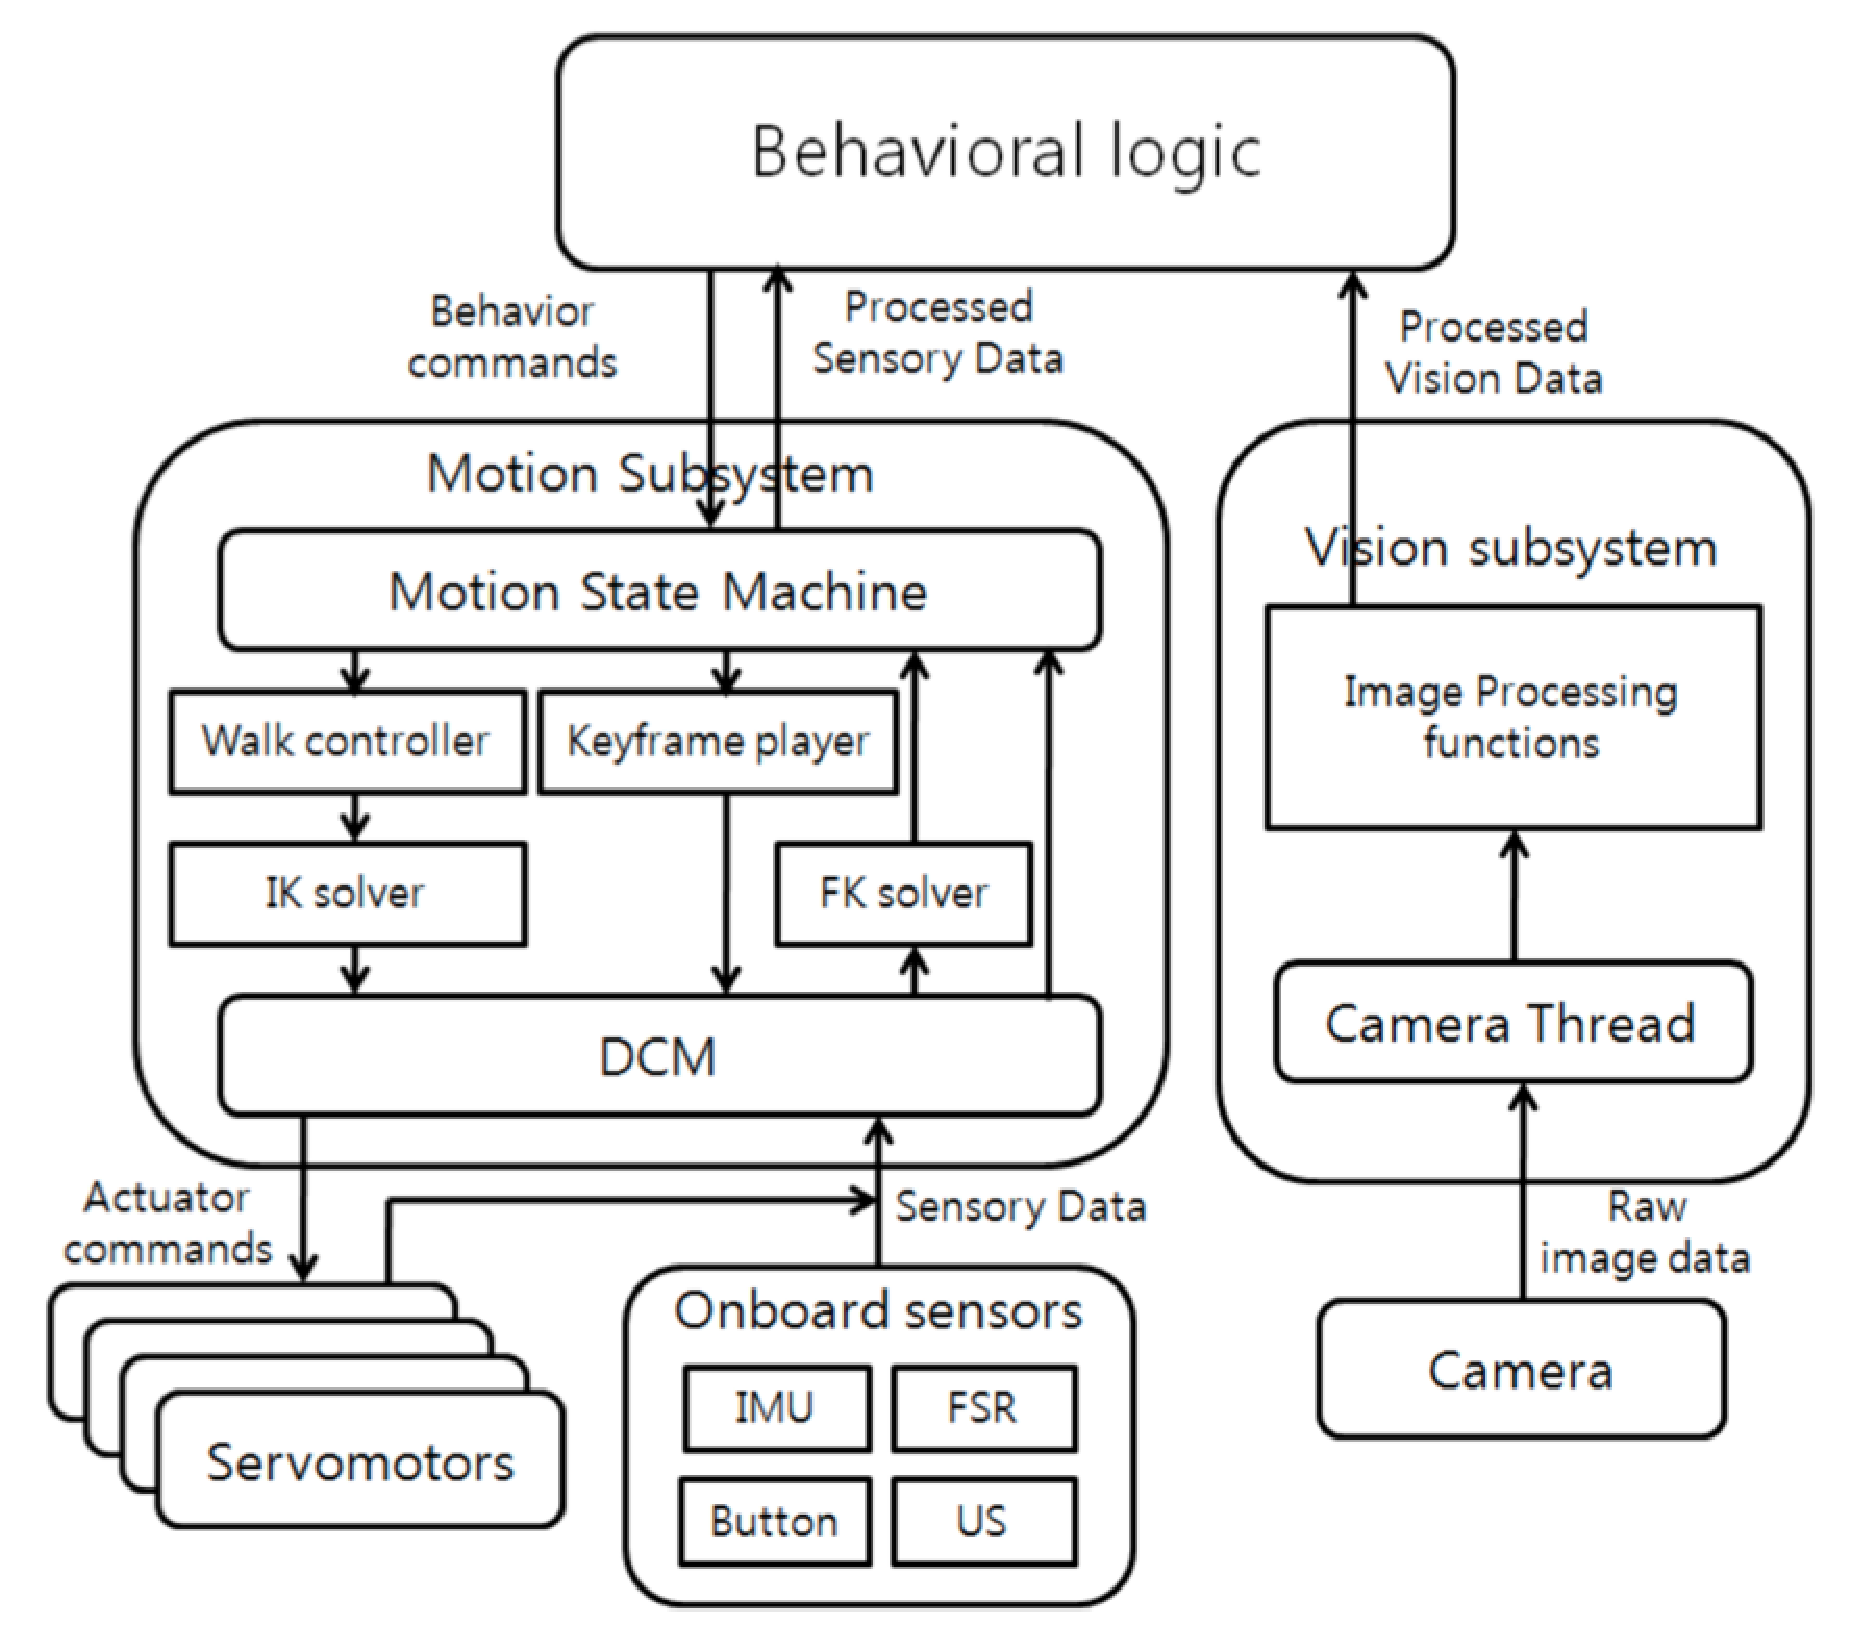
\includegraphics[width=1.0\textwidth]{figures/SoftArchOverview.eps}
		\caption{Block Diagram of the Software Architecture.}
		\label{fig:softarch}
	\end{figure}

	Inter-process communication is accomplished via shared memory. Important information such as ball distance, position on the field, and game state are examples of shared memory variables. Any module can write and read to shared memory. In addition, any operator connected to a Nao via secure shell can monitor the data stored in the shared memory module without any change or impact on the running system, allowing for real-time on-the-fly debugging and analysis through either Lua or MATLAB.

	The main modules accessed by our Lua routines are as follows, layered hierarchically:
	\begin{description}
		\item[Camera] Direct interface to the cameras located in the forehead (upper) and mouth (lower); controls switching frequency and bundling of images in YUYV format.
  		\item[Vision] Interprets incoming images; based on the user-created color table and camera parameters, the module passes on information relating to the presence and relatively location of key objects such as the ball, defending goal posts, attacking goal posts, field lines, field corners, and other robots.
	  	\item[World] Models the robot's state on the field, including pose and filtered ball position; 
		\item[Body] Handles physical sensory information and functions; reads joint encoders, IMU data, foot weight sensors, battery voltage, and chest button presses, but can also set motor positions, stiffnesses, and LED's.
  		\item[Motion] Dictates general movements on the Nao; i.e. sitting, standing, diving	
	  	\item[Walk] Controls omni-directional locomotion; takes in hand-tuned parameters and applies them to a zero-moment point (ZMP) based walk engine.
		\item[Kick] Maintains intra-robot stability during kick movements; different kick settings can be loaded to allow for powerful standing kicks, quick walk-kicks, and decisive side-kicks.
  		\item[Keyframes] Lists scripted positions for certain movements; getting up from front and back falls is done by feeding the Body module a series of motor positions and timings.
	  	\item[Game State Machine] Receives and relays information from the Game Controller; information from the GSM such as game state determines behavior among all robots on the field during certain times of the game.
		\item[Head State Machine] Controls head movements; different conditions determine when to switch into ball searching, ball tracking, and simply looking around.
  		\item[Body State Machine] Dispatches movement instructions; conditions from all previous modules will cause the Nao to switch between chasing after far away balls, performing curved approaches to line up for shots, dribbling, and performing kicks when the ball is close enough.
	  \end{description}



\section{Motion}
	Motion is controlled by a dynamic walk module combined with predetermined scripted motions. One main development has been a bipedal walk engine that allows for fast, omni-directional motions. IMU feedback is used to modulate the commanded joint angles and phase of the gait cycle to provide for further stability during locomotion. In this way, minor disturbances such as carpet imperfections and bumping into obstacles do not cause the robot to fall over. The robot has several powerful kick motions using pre-defined keyframes and a ZMP walk-kick for quicker reaction. Keyframes are also used for all of the get-up motions under different battery levels.

\subsection{Walk}

	\begin{figure}[H]
		\centering
		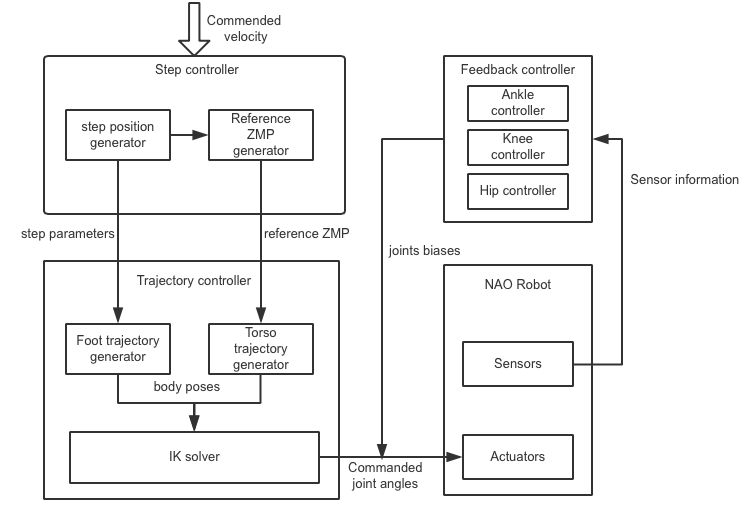
\includegraphics[width=1\textwidth]{figures/WalkOverView.png}
		\caption{Overview of the walk controller}
	\end{figure}

	The walk engine generates trajectories for the robot's center of mass (COM) based upon desired translational and rotational velocity settings. The module then computes optimal foot placement given this desired body motion. Inverse kinematics (IK) are used to generate joint trajectories so that the zero moment point (ZMP) is over the support foot during the step. This process is repeated to generate alternate support and swing phases for both legs.

\subsubsection{Step controller}
	The step controller determines the parameters of each step give different commended velocity and hardware parameters. Each step is defined as 

	\begin{eqnarray*}
		STEP_i=\{SF,t_{step},L_i,T_i,R_i,L_{i+1},T_{i+1},R_{i+1}\}
	\end{eqnarray*}
	
	where SF denotes the support foot, $t_{step}$ is the duration of the step, $L_i,R_i,T_i$ and $L_{i+1},R_{i+1},T_{i+1}$ are the initial and final 2D poses of left foot, right foot and torso. $L_i,R_i,T_i$ are the final poses from the last step, $L_{i+1},R_{i+1}$ are calculated using the commended velocity. Foot reachability and self-collision constraints are also considered given different configurations in the pre-defined walk setting file, as shown below.

	\begin{figure}[H]
		\centering
		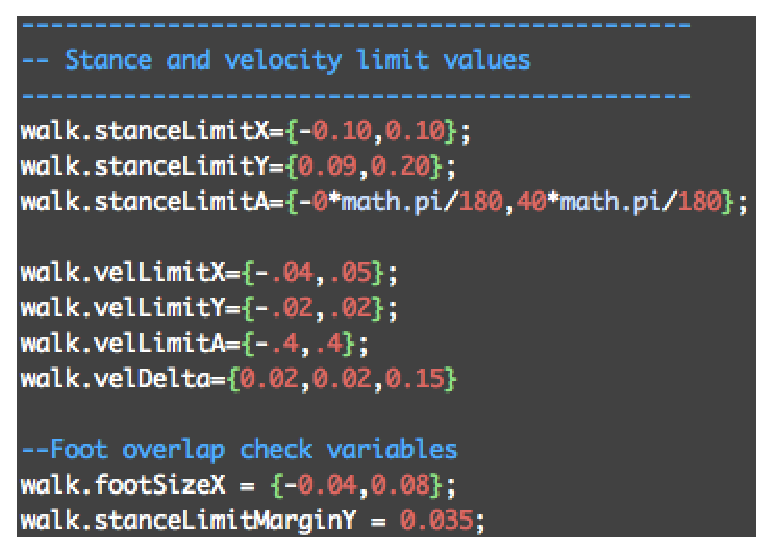
\includegraphics[width=.60\textwidth]{figures/WalkFile.eps}
		\caption{Example parameters for one of our walk files.}
	\end{figure}

	To get the most stable posture, the center of mass should lies on the middle point of two feet. Thus the target torso pose $T_{i+1}$ is set to the midpoint of $L_{i+1}$ and $R_{i+1}$.
Given the initial and final position of the feet and torso, the reference ZMP trajectory $p_i(\phi)$ as the following piecewise-linear function for the left support case
$$ p_i(\phi)=\left\{
\begin{array}{rcl}
T_i(1-\frac{\phi}{\phi_1})+L_i \frac{\phi}{\phi_1} & & 0 \leq \phi < \phi_1\\
L_i & & \phi_1 \leq \phi < \phi_2\\
T_i(1-\frac{1-\phi}{1-\phi_2})+L_i \frac{1-\phi}{1-\phi_2} & & \phi_2 \leq \phi < 1\\
\end{array} \right. $$
where $\phi$ is the walk phase and $\phi_1,\phi_2$ are the timing parameters determining the duration of single support phase and double support phase.

\subsubsection{Trajectory controller}
	The trajectory controller generates torso and foot trajectories for the current step. We first define $\phi_{single}$ as the single support walk phase
$$ \phi_{single}=\left\{
\begin{array}{rcl}
0 & & 0 \leq \phi < \phi_1\\
\frac{\phi-\phi_1}{\phi_2-\phi_1} & & \phi_1 \leq \phi < \phi_2\\
1 & & \phi_2 \leq \phi < 1\\
\end{array} \right. $$
We then define a parameterized trajectory function
$$f_x(\phi)=\phi^{\alpha}+\beta \phi(1-\phi)$$
to generate the foot trajectories
$$L_i(\phi_{single})=L_{i+1}f_x(\phi_{single})+L_i(1-f_x(\phi_{single}))$$
$$R_i(\phi_{single})=R_{i+1}f_x(\phi_{single})+R_i(1-f_x(\phi_{single}))$$
The torso trajectory $x_i(\phi)$ is calculated by modeling the robot as a inverted pendulum. Thus
$$p=x-t_{ZMP}\ddot x$$
With the reference ZMP trajectory we defined before, the $x_i(\phi)$ during the step with zero ZMP error should be
$$ x_i(\phi)=\left\{
\begin{array}{rcl}
p_i(\phi)+a_i e^{\frac{\phi}{\phi_{ZMP}}}+b_i e^{-\frac{\phi}{\phi_{ZMP}}}-\phi_{ZMP}m_i sinh \frac{\phi-\phi_1}{\phi_{ZMP}}& & 0 \leq \phi < \phi_1\\
p_i(\phi)+a_i e^{\frac{\phi}{\phi_{ZMP}}}+b_i e^{-\frac{\phi}{\phi_{ZMP}}} & & \phi_1 \leq \phi < \phi_2\\
p_i(\phi)+a_i e^{\frac{\phi}{\phi_{ZMP}}}+b_i e^{-\frac{\phi}{\phi_{ZMP}}}-\phi_{ZMP}n_i sinh \frac{\phi-\phi_1}{\phi_{ZMP}} & & \phi_2 \leq \phi < 1\\
\end{array} \right. $$
where $phi_{ZMP}=t_{ZMP}/t_{STEP}$. $m_i,n_i$ are ZMP slopes defined as following for left support case
$$m_i=\frac{L_i-T_i}{\phi_1},\;\;n_i=-\frac{L_i-T_{i+1}}{1-\phi_2}$$
and for right support case
$$m_i=\frac{R_i-T_i}{\phi_1},\;\;n_i=-\frac{R_i-T_{i+1}}{1-\phi_2}$$
$a_i,b_i$ can then be calculated given the boundary condition $x_i(0)=T_i$ and $x_i(1)=T_{i+1}$. The resulting ZMP and torso trajectory are shown below

\begin{figure}[H]
		\centering
		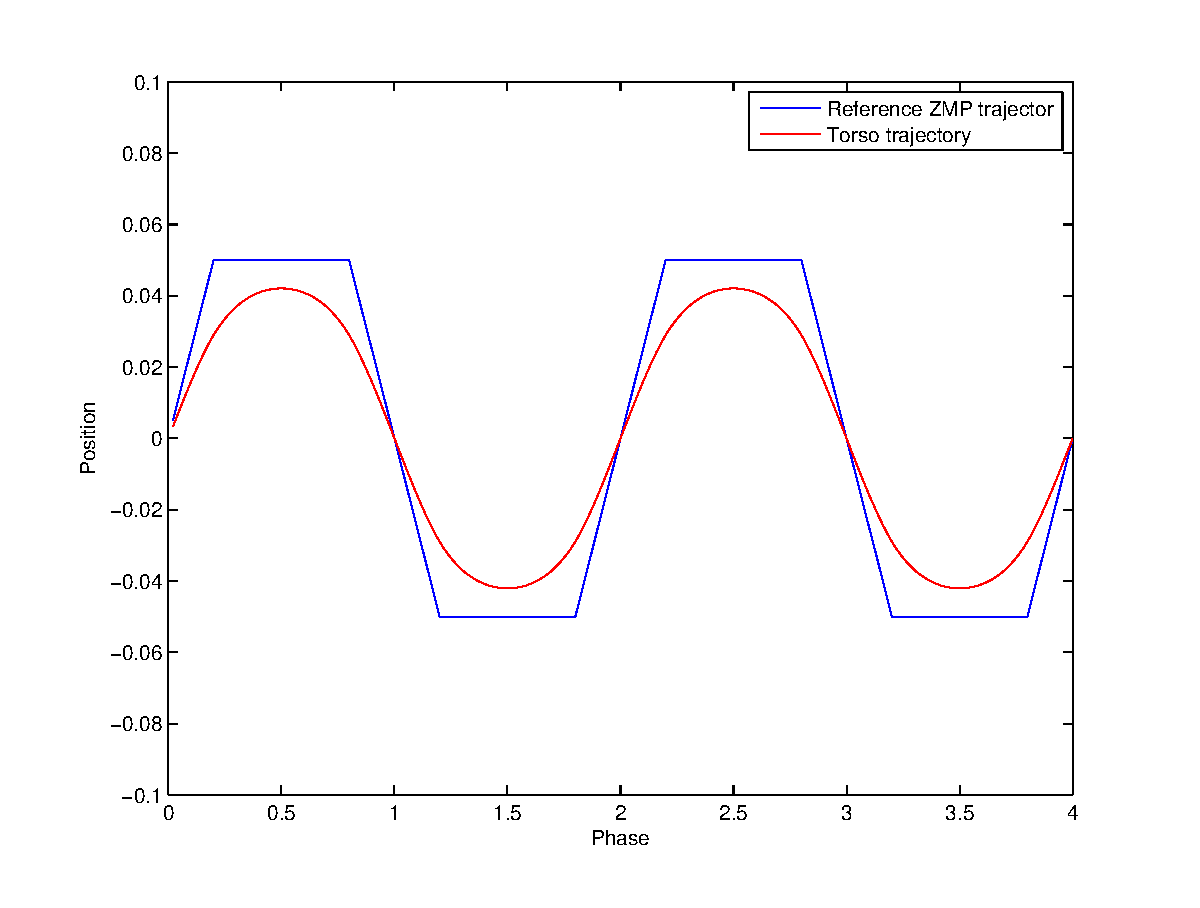
\includegraphics[width=1\textwidth]{figures/ZMP.eps}
		\caption{An example for a reference ZMP trajectory and corresponding torso trajectory.}
	\end{figure}
Given body pose and feet poses, an inverse kinematics module is used to calculate angles for each joints so that the robot can actually walk as desired.

\subsubsection{Feedback controller}
	The feedback controller takes in the sensor information from the robot during the walk and tries to stabilize it by controlling the ankle joints, knee joints and hip joints. Roll and pitch angles are used as inputs for several simple PD controllers. Knee and hip joints are used to overcome pitch errors while ankle joints are used for roll error. If the pitch angle or roll angle is higher than a threshold, the walk motion will be stopped. This can be caused by other robot pushing our robot during a game.   
  
\subsection{Kicks}
	  Our kicks this year are a combination of scripted keyframes and ZMP-based kicks. Of our three kicks -- standing, walk, and side -- only the walk-kick utilizes the new ZMP engine. The old-fashioned style kicks are created by specifying motor positions and timings, and must be carefully tuned by hand in order to ensure balance, stability, and power. The new kicks are inherited from our merge with Team DARwIn. Similar to how the walk engine calculates joint positions in response to motion requests of the COM and ZMP, the newer kick calculates the way that the robot needs to balance in order to perform faster and more powerful kicks.  
\begin{comment}
	  While we utilized a mix of a keyframed standing and keyframed walk-kick during the US Open to great success, after transitioning to the ZMP walk-kick, we used this newer kick solely during our matches in Eindhoven. This allowed us to have greater control over the ball, and react quicker than opponent robots which would approach a ball and take excessive time during their keyframe motions to do a kick.
\end{comment}
  
\subsection{Get up}
	Get up motions are all defined by several keyframe files. A keyframe file consists of a series of frames, snapshots of the 22 motor positions along with a timing by which those positions must be reached from the previous frame. Though the motors natively read and write radians to their encoder, we use degrees and convert them later for better readability.
	
	\begin{lstlisting}
  	  	angles = vector.new({
	  		0.1, 25.5,
		  	109.8, 11.0, -88.9, -21.4,
  			-13.7, -0.3, 17.1, -5.6, 5.2, 7.6,
	  		0.0, -1.8, 14.6, -1.1, 4.9, -2.7,
		  	109.9, -10.2, 88.7, 19.9,
  	  	})*math.pi/180,
	duration = 0.400;
	\end{lstlisting}

  	The motors in order are:

	\begin{multicols}{3}
		\begin{enumerate}
			\item HeadYaw
  			\item HeadPitch
	  		\item LShoulderPitch
		  	\item LShoulderRoll
			\item LElbowYaw
  			\item LElbowRoll
	  		\item LHipYawPitch
		  	\item LHipRoll
			\item LHipPitch
  			\item LKneePitch
	  		\item LAnklePitch
		  	\item LAnkleRoll
			\item RHipYawPitch
  			\item RHipRoll
	  		\item RHipPitch
		  	\item RKneePitch
			\item RAnklePitch
  			\item RAnkleRoll
	  		\item RShoulderPitch
		  	\item RShoulderRoll
			\item RElbowYaw
  			\item RElbowRoll
		\end{enumerate}
	\end{multicols}

	These keyframes are hand-tuned based upon experimentation. To prolong the life of our robots, we do most of the heavy keyframe testing in Webots and then port it to the robots and perform final checks to verify full functionality. Some keyframes can make the robot get up is 6 seconds, which is much faster than some other get up motions. However, the get up motion performance is highly depending on the battery level and the hardware condition. During the test, many robots cannot get up with fast motions if their battery levels are lower than 8, or if they have a broken joint. To avoid keep picking up our robots during a real game because they cannot get up, we set each robot to have two get up motions. The default get up motion is set to be the fast one. If the battery level is lower than a threshold, or the robot have failed to get up once, it will switch to the slow get up motion. This change helped us a lot in Joao Pessoa. 



\section{Cognition}
	The cognition module acquires visual information from cameras and returns locations of key objects on the field, as well as the position of the robot itself. Figure \ref{fig:cog} shows the framework of the cognition module. 

	\begin{figure}[H]
		\centering
		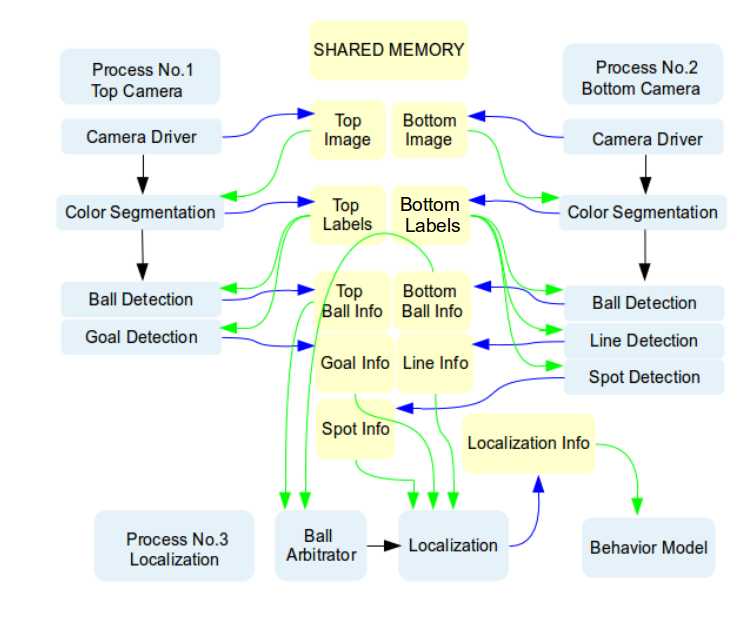
\includegraphics[width=1.0\textwidth]{figures/CogStructure.png}
		\caption{Block Diagram of the Cognition Module.}
  		\label{fig:cog}
	\end{figure}

	Each Aldebaran Nao robot has two cameras on board, also know as the top (forehead) and bottom (mouth) camera. They feed images in stream at 30 frames per second each. Images from the top and bottom cameras are processed simultaneously by two processes. Different object detection routines are run on images from different cameras to improve efficiency. An arbitrator process coordinates intermediate results from the two processes and runs the localization module. The final results from the cognition module are sent to behavior controls.

\subsection{Image Processing}
	Algorithms used for processing visual information are the same for both camera processes, and they are similar to those used by other Robocup teams. 

	The first step is color segmentation. A Gaussian mixture model is used to partition the YCbCr color cube into seven colors:

	\begin{itemize}
		\item Orange (Ball)
		\item Yellow (Goals)
		\item Green (Field)
		\item White (Lines)
		\item Pink (Robot Jerseys)
		\item Blue (Robot Jerseys)
		\item Black (Others)
	\end{itemize}

	The actual calibration process follows a supervised learning routine: images taken from both cameras are trained to form a color look-up table. While the robot is running, the image processing pipelines segment raw images into discretely colored images by classifying individual pixels based upon their mapped values in the color table. The segmented images are further shrunk to lower-resolution colored labels by merging adjacent pixels. Figure \ref{fig:unprocessed} to \ref{fig:labelb} show each step of color segmentation.

	\begin{figure}[H]
		\centering
		\subfigure[Raw Image]{
			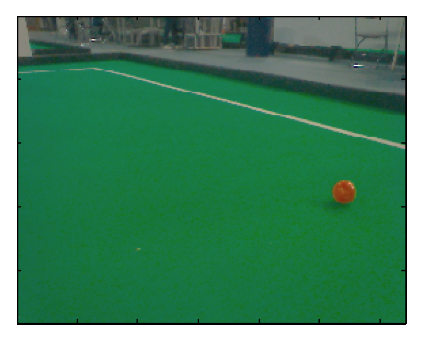
\includegraphics[width=.6\textwidth]{figures/Unprocessed.eps}
    			\label{fig:unprocessed}
		}
    		\quad
		\subfigure[Segmented Image]{
  	  		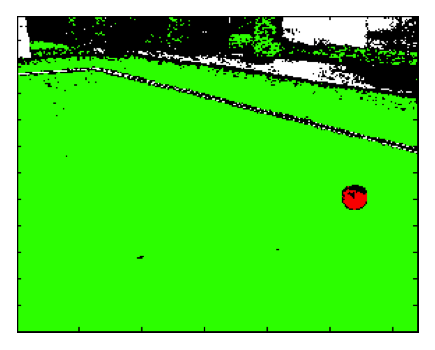
\includegraphics[width=.4\textwidth]{figures/Processed.eps}
			\label{fig:processed}
		}
    		\quad
 		\subfigure[Colored Label]{
			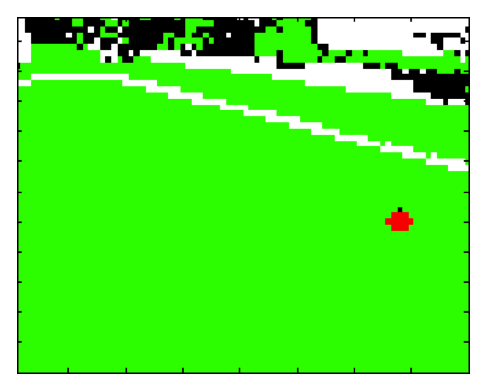
\includegraphics[width=.4\textwidth]{figures/LabelB.eps}
    			\label{fig:labelb}
		}
  	      \caption{}
	\end{figure}



	The next step is object detection on colored labels. Connected regions are recognized as either connected components or edge regions, and objects are recognized from the statistics - such as the bounding box of the region, the centroid location, and the chord lengths in the region - of the colored regions. In this manner, the location of the ball and goal posts are detected. 

	Field line recognition follows a slightly more complicate routine. Once all white pixels surrounded by green are located, a Hough transform is used to search for relevant line directions. In the Hough transform, each possible line pixel \((x, y)\) in the image is transformed into a discrete set of points \((\theta_{i},r_{i})\) which satisfy:
  
	\begin{equation}
		x \cos \theta_{i} + y \sin \theta = r_{i} 
	\end{equation}

	The pairs \((\theta_{i},r_{i})\) are accumulated in a matrix structure where lines appear as large values as shown in Figure \ref{fig:Hough}. After these lines are located, they are identified as either interior or exterior field lines based upon their position.

	\begin{figure}[H]
		\centering
		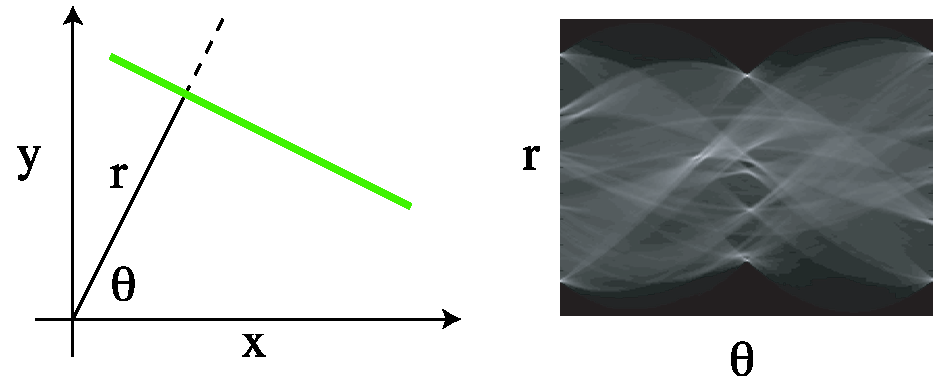
\includegraphics[width=0.8\textwidth]{figures/Hough.eps}
		\caption{Hough transformation for field line detection in images.}
  		\label{fig:Hough}
	\end{figure}

\subsection{More Details on Object Detection - Chris \& Junda}


\subsubsection{Goalpost Detection}


\subsubsection{Line Detection}


\subsubsection{Ball Detection}


\subsection{Self-Localization}
	The problem of knowing the location of robots on the field is handled by a probabilistic model incorporating information from visual landmarks such as goals and lines, as well as odometry information from the effectors. Recently, probabilistic models for pose estimation such as extended Kalman filters, grid-based Markov models, and Monte Carlo particle filters have been successfully implemented. Unfortunately, complex probabilistic models can be difficult to implement in real-time due to a lack of processing power on robots. This issue is addressed with a pose estimation algorithm that incorporates a hybrid Rao-Blackwellized representation that reduces computational time, while still providing a high level of accuracy. The algorithm models the pose uncertainty as a distribution over a discrete set of heading angles and continuous translational coordinates. The distribution over poses \((x,y,\theta)\), where \((x,y)\) are the two-dimensional translational coordinates of the robot on the field, and $\theta$ is the heading angle, is first generically decomposed into the product:

	\begin{equation}
		P(x,y,\theta) = P(\theta)P(x,y|\theta) = \sum\limits_{i} P(\theta_{i})P(x,y,|\theta_{i})
	\end{equation}

 	The distribution $P(\theta)$ is modeled as a discrete set of weighted samples $\{\theta_{i}\}$, and the conditional likelihood $P(x,y|\theta)$ as simple two-dimensional Gaussian. This approach has the advantage of combining discrete Markov updates for the heading angle with Kalman filter updates for translational degrees of freedom.

	\begin{figure}[H]
		\centering
		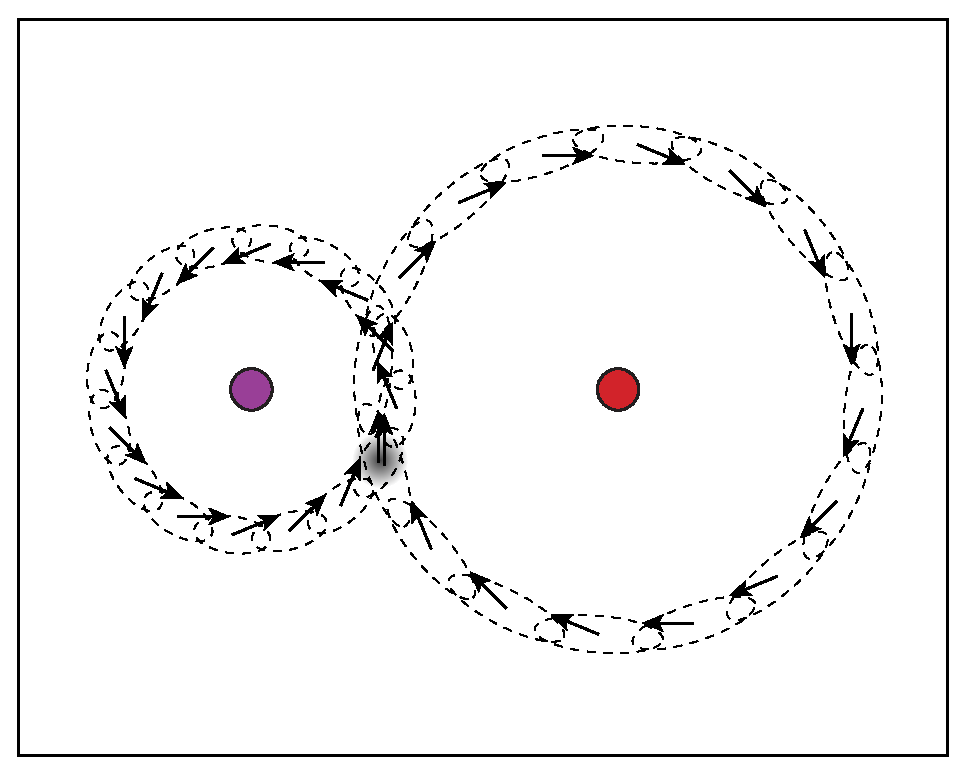
\includegraphics[width=.6\textwidth]{figures/RaoBlackwell.eps}
		\caption{Rao-Blackwellized probabilistic representation used for localization.}
		\label{fig:raoblack}
	\end{figure}
 
	This algorithm enables robots to quickly incorporate visual landmarks and motion information to consistently estimate both the heading angle and translation coordinates on the field as shown in Figure \ref{fig:raoblack}. Even after the robots are lifted ('kidnapped') by the referees, they will quickly re-localize their positions when they see new visual cues.	

\subsubsection{Particle Initialization}
	The localization algorithm utilizes 200 particles to estimate the position of the robot. Properly initializing the positions of the particles helps improve the accuracy of the localization algorithm. Before the game starts, the particles are initialized on the sides of the defending half of the field, as shown in Figure \ref{fig:Init}. In the Set state, if the robot is not manually replaced, its particles are initialized near the possible initial positions defined in our game strategy. Besides, during the game, when a robot falls down, its localization particles' heading angles are reinitialized.
    
	\begin{figure}[H]
		\centering
		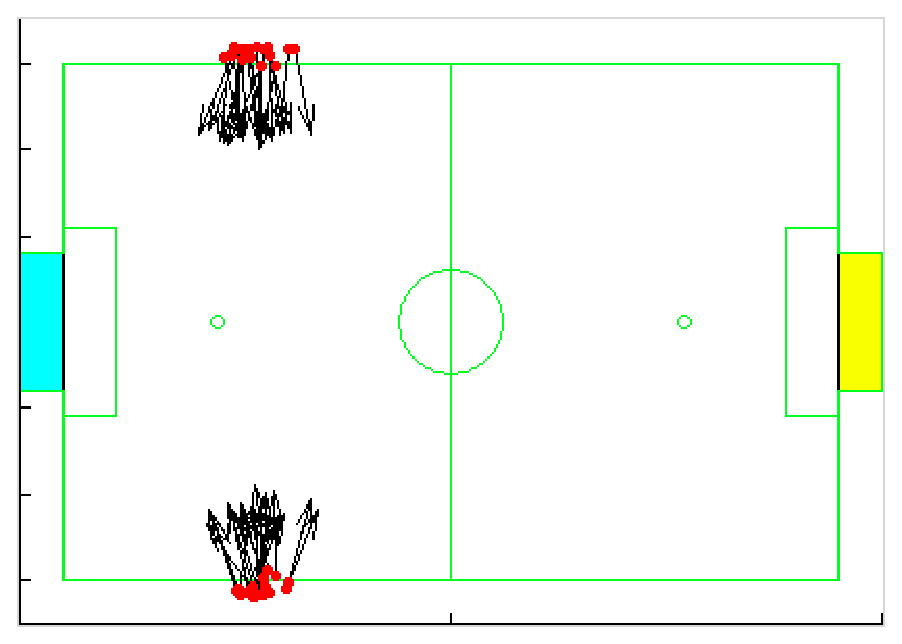
\includegraphics[width=0.6\textwidth]{figures/InitParticles}    
		\caption{Initialization of particles before game starts.}
		\label{fig:Init}
	\end{figure}

\subsubsection{Odometry, Landmark Observation and Re-sampling}
	A Kalman filter is implemented to track the continuous change on the position and weight of each particle. The filtering is a product of two steps: the motion model update and the measurement update. The motion model update - also referred to as the odometry update - utilizes the robot kinematics to update the particle filter as the robot walks around the field. Given the joint angles of the robot, forward kinematics is used to compute the location of the robot's feet as it walks. The change in translation and rotation of the body of the robot are computed based on the position of the feet, as shown in Figure \ref{fig:odometry}, and used to update the particle filter.

	\begin{figure}[H]
		\centering
		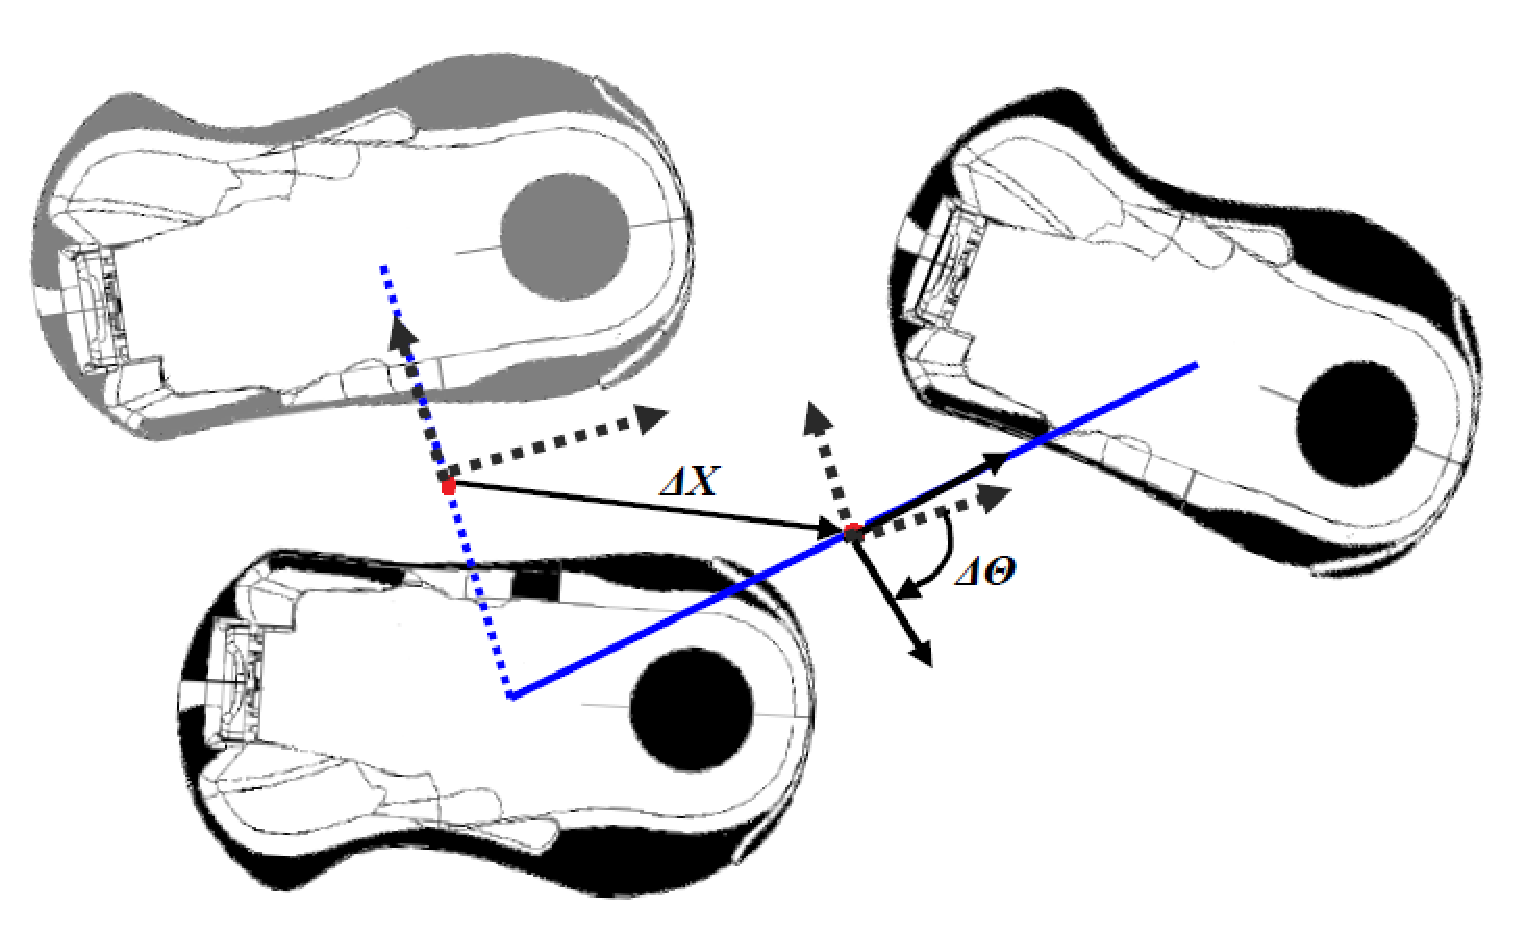
\includegraphics[width=0.6\textwidth]{figures/Odometry.eps}
		\caption{Visualization of the odometry calculation after one step.}
		\label{fig:odometry}
	\end{figure}a set of camera parameter values. These parameters should make the top and bottom camera visually appear as similar as possible because both

	The measurement model refines this estimate using sensory inputs, such as vision-based landmark detection.  The measurement model incorporates positions of landmarks to adjust the particle positions and their weights in the filter. Positions of landmarks are weighted based upon their reliability. For instance, goal post detection is considered convincing and used to correct both the position and the direction of the robot. Meanwhile, corner and line detections are only used to correct the direction due to large variance in their position calculation.

	The algorithm re-samples every 0.1 seconds. A stratification method is used to redraw all  particles so that the ones with higher weight will stay. Figure \ref{fig:particlesafter} illustrate the result of self-localization.

	\begin{figure}[H]
		\centering
		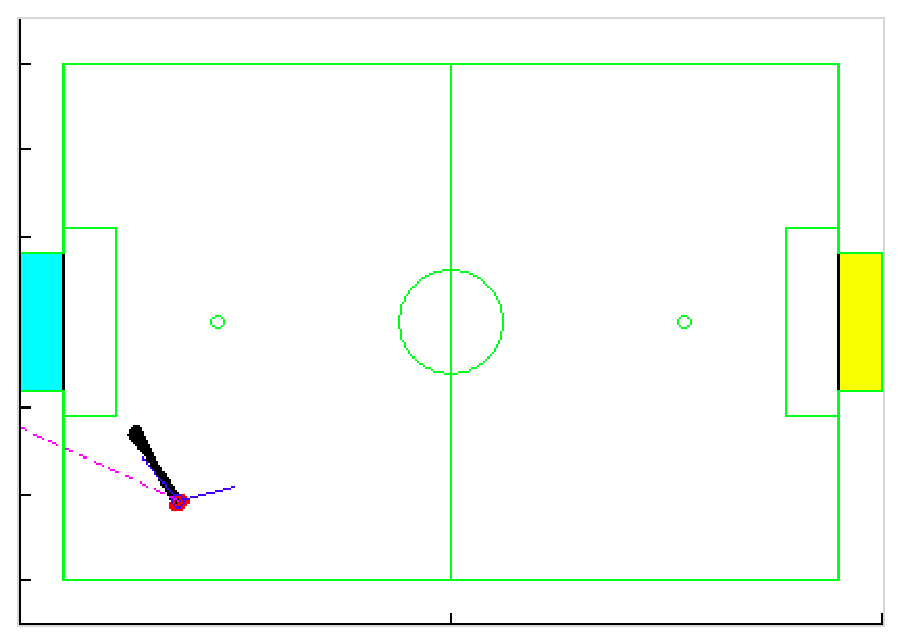
\includegraphics[width=.6\textwidth]{figures/FocusedParticles.eps}
	  	\caption{The robot weighs different landmark positions to establish an accurate estimation of its position on the field.}
		\label{fig:particlesafter}
  	\end{figure}

\subsubsection{Error Correction}
	One great challenge with self-localization in the Standard Platform League is the symmetric field. Under ideal circumstances where the robot's starting position is known, the basic particle filter approach alone is enough to keep track of the correct robot pose. However, noise in the motion model, inevitable false positive detections of landmarks, and falling down, will all eventually cause the robot to converge on a pose that is symmetrically opposite the true location. A team correcting mechanism based on goalie ball information is introduced.

	Since the goalie mostly stays in penalty box and close to the defending goal posts, it should be more confident about the location of itself and the ball than other robots on field. The correcting mechanism works when a player robot and the goalie see the ball simultaneously but believe the ball is on different sides of the field. Under such circumstances, it is very likely that the player robot's localization is flipped and its particles will be flipped back against the center of the field.

	Moreover, robots are very likely to generate localization error when they fall over near the center of the field. The correcting mechanism labels these robots as "confused players", which will not make direct shots to goal. Instead, they will dribble or slightly kick the ball until the goalie sees the ball and confirms their positions.

\subsection{Debugging Tools}
\subsubsection{Monitoring}    
	It is crucial that developers know what the robot perceives at each stage of cognition. The monitor program is designed for this purpose. It receives data packets from an active robot and display them. The transmitted data include:
	
	\begin{itemize}
		\item{System Time Stamps}
		\item{Images}
		\item{Color-segmented Images}
		\item{Location of Itself and Objects}
		\item{Cognition-related Shared Memory}
	\end{itemize}

	A GUI is designed to display these information, as shown in Figure \ref{fig:monitor}. Developers can view the images (raw and segmented) from both on-board cameras and eye-ball check the correctness of object detections. Important debug messages are listed on the right side to provide more information on details of the cognition process.

      \begin{figure}[H]
		\centering
    		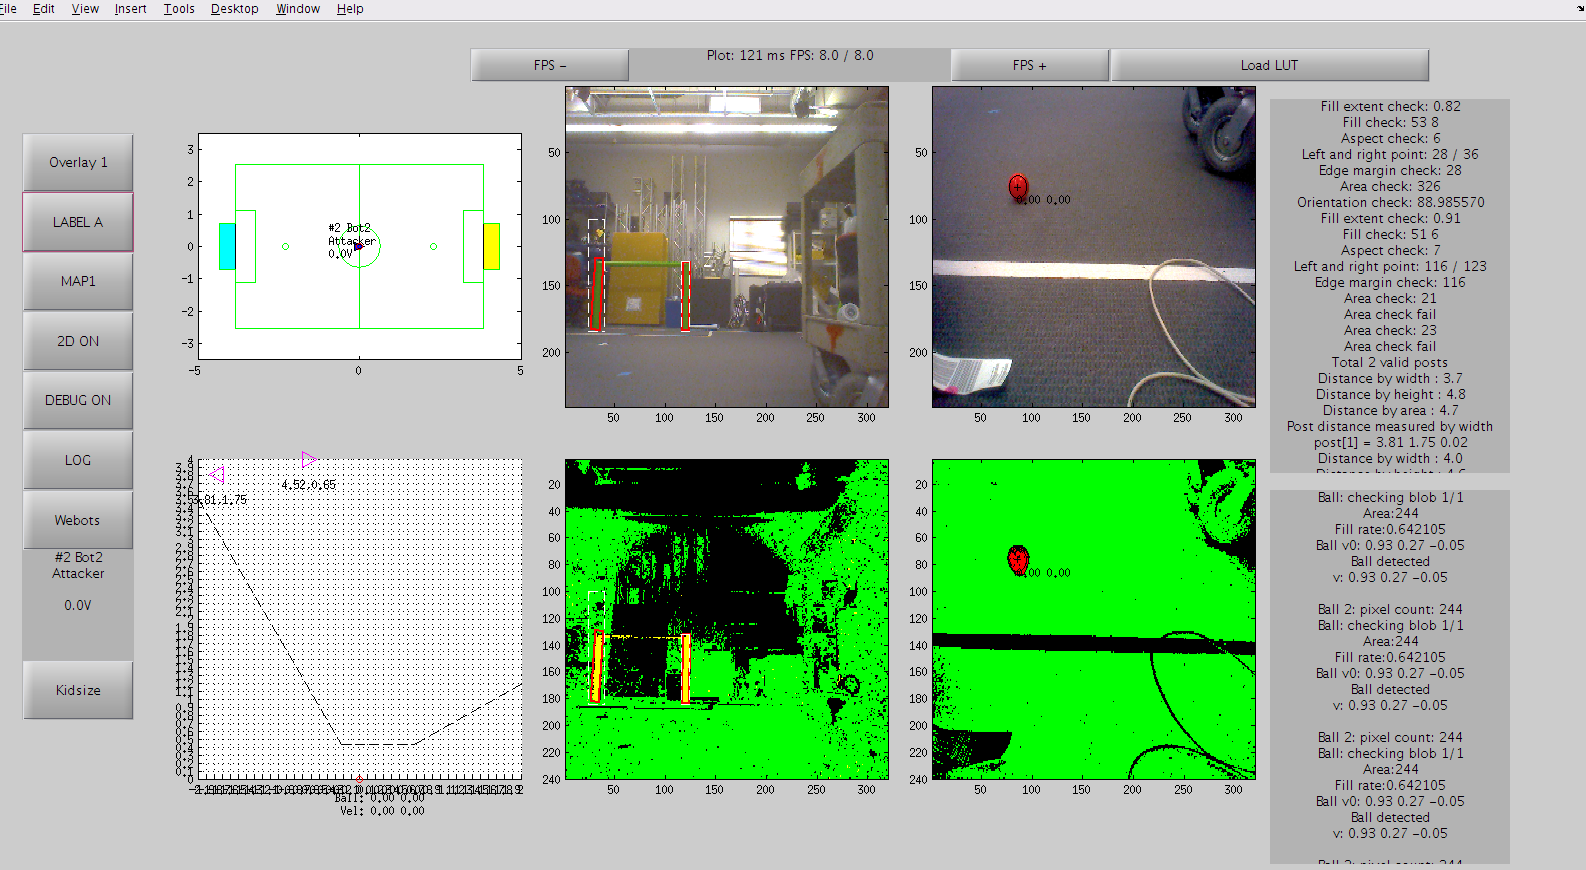
\includegraphics[width=1.0\textwidth]{figures/Monitor.png}
		\caption{Monitor}
    		\label{fig:monitor}
	\end{figure}

	The monitor also supports logging functionality, which stores the real time cognition information in a local file.
A vision simulator is designed to open and run image processing on these log files. As the result, debugging can be done off-line from a robot, which greatly improves development efficiency.
 
\subsubsection{Camera Calibrator}
      Since cognition depends highly on the quality of images from the cameras, calibrating the camera parameters (i.e. Exposure, Contrast, and Saturation) is an important task. A script is written to facilitate the process. During calibrating, developers can change camera parameters by key presses and check the quality of images through the Monitor program. Figures \ref{fig:topparams} and \ref{fig:bottomparams} are screen shots of the script.
 	    
	\begin{figure}[H]
    		\centering
		\subfigure[Top camera]{
    			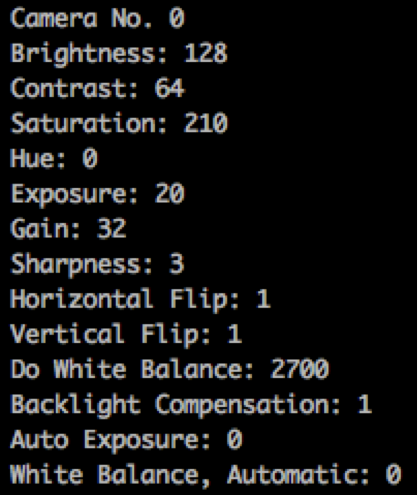
\includegraphics[width=.3\textwidth]{figures/TopCamParams.png}
			\label{fig:topparams}
    		}
		\quad
    		\subfigure[Bottom camera]{
			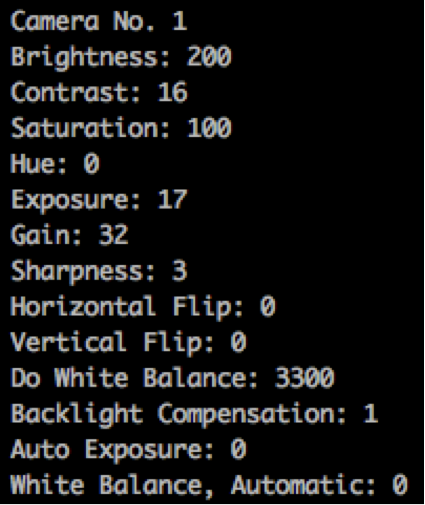
\includegraphics[width=.3\textwidth]{figures/BottomCamParams.png}
			\label{fig:bottomparams}
    		}
		\quad
    		\caption{Example camera parameters.}	
	\end{figure}

\subsubsection{Colortable Tool}
	The quality of color segmentation is also a key factor for successful cognition process. Therefore, another calibration tool is required to build robust color look-up tables. The colortable tool loads in logged images from the on-board cameras for developers to manually train the color. Developers can monitor the quality of the colortable throughout the calibration process. Figure \ref{fig:colortable} is a screen shot of the tool.

	\begin{figure}[H]
		\centering
		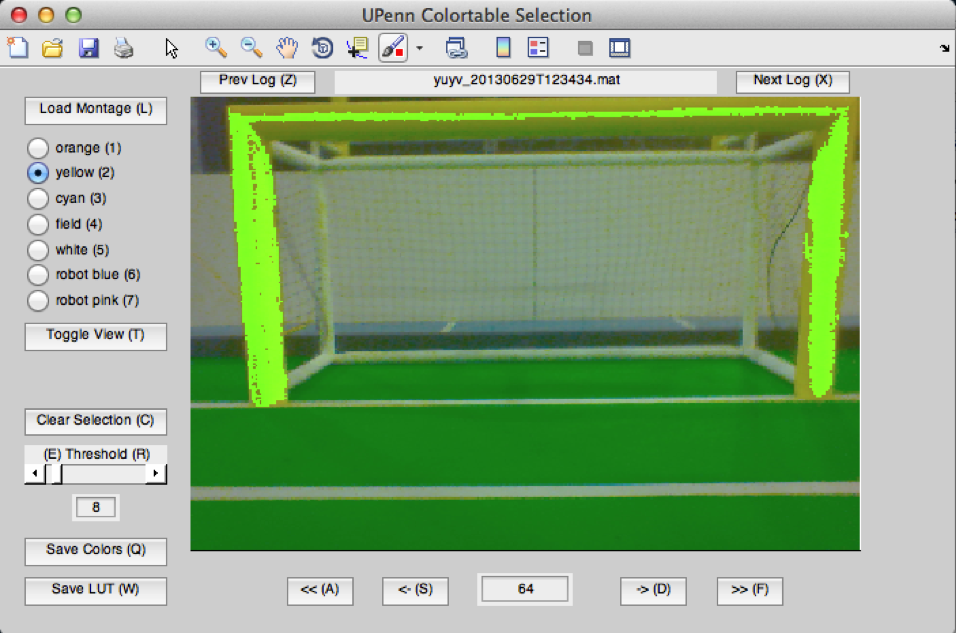
\includegraphics[width=.6\textwidth]{figures/ColorSelectionTool.png}
		\caption{The Colortable Tool}
		\label{fig:colortable}
	\end{figure}



\section{Behavior}
	Finite state machines (FSMs) dictate the behaviors robots and allow them to adapt to constantly changing conditions on the field.  The implementation of an FSM consists of a series state definitions and one arbitrator file that defines the transitions between states. 

	Each state consists of three stages:  \texttt{entry}, \texttt{update} and \texttt{exit}. The \texttt{entry} and \texttt{exit} stages specify actions to be taken when the robot first enters a state or finally completes a state. During the \texttt{update} stage, which is in between, the robot constantly cycles through a routine. Usually it moves on the field while querying cognition information, until certain conditions are met. For instance, in state \textit{BodySearch}, the robot rotates in place until either it detects the ball or it times out after not seeing the ball for 5 seconds. In the first case, it transits into a state of chasing the ball; in the other case, the robot transits into a state of going to the center of the field (where it has a better chance of detecting the ball).

\subsection{The Body Finite State Machine }
	The Body Finite State Machine (BodyFSM) is the main behavior control module. It regulates robot movements and kicks during the game. Two sets of state machines are implemented, one for normal players and the other for the goalie. The key difference is that the goalie needs hold its position and stay in the penalty box in most cases while field players need to walk around and chase the ball.

\subsubsection{BodyFSM for Normal Players}	
	Figure \ref{fig:bodyfsm} shows the transitions of states for a normal robot player. It is followed by brief descriptions of the states. The basic routine is: \texttt{Search for ball} $\to$ \texttt{Approach the ball} $\to$ \texttt{Dribble of Make a Shot}.
		
	\begin{figure}[H]
		\centering
		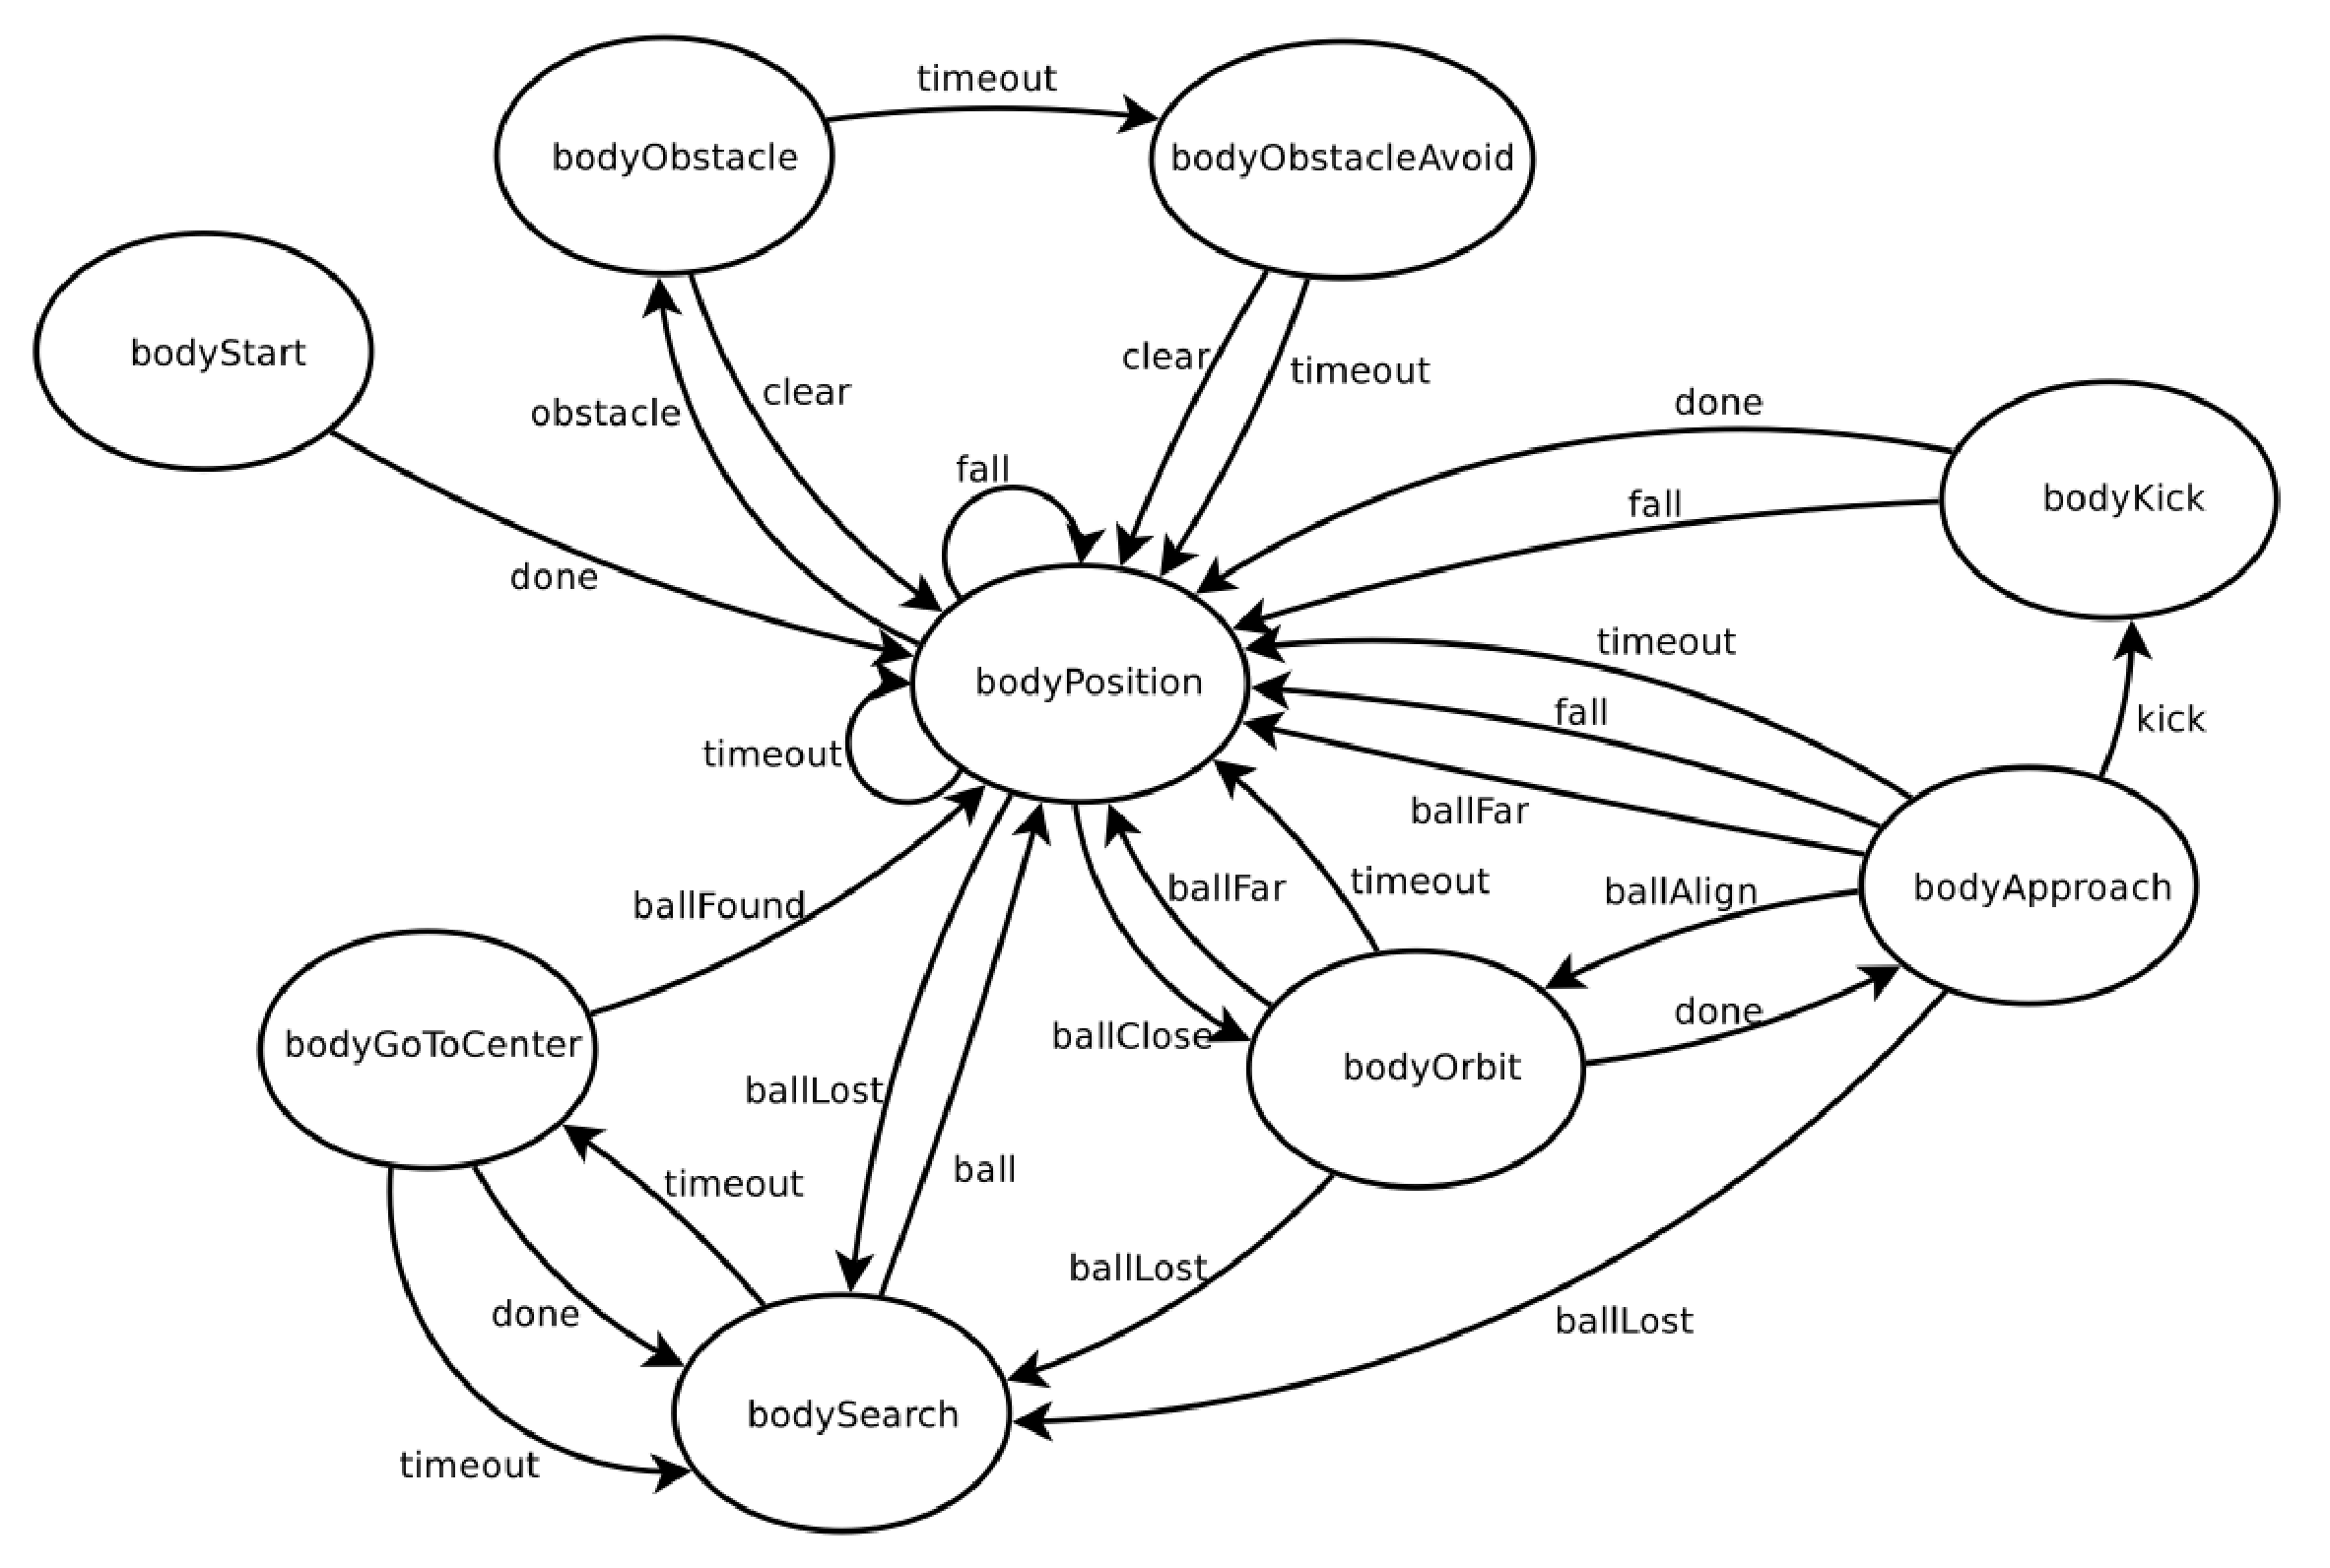
\includegraphics[width=\textwidth]{figures/BodyFSM.eps}
		\caption{Body State Machine for a non-goalie player.}
		\label{fig:bodyfsm}
	\end{figure}
		
	\begin{multicols}{2}
		\begin{description}
			\item[bodyApproach] Align for kick.
			\item[bodyChase] Ball sighted; run for ball and slow as distance decreases.
			\item[bodyDribble] Dribble the ball.
			\item[bodyGotoCenter] Return to the center of the field.
			\item[bodyKick] Perform a standing kick.
			\item[bodyObstacle] Obstacle detected.
			\item[bodyObstacleAvoid] Sidestep or stop movement until the obstacle clears.
			\item[bodyOrbit] Make fine adjustments to trajectory before kicking.
			\item[bodyPosition] Main body state; most states will transition back here.
			\item[bodySearch] Revolve and search for the ball.
			\item[bodyStart] Initial state when the main code is started up. 
			\item[bodyStop] Stops the robot completely.
			\item[bodyWalkKick] Perform a kick while in motion.
			\item[bodyUnpenalized] Commands the robot to stand back up and walk into the field after being unpenalized.
		\end{description}
	\end{multicols}

	One important note on BodyFSM is the approaching method. The simplest implementation is to make the robot walk straight to the ball and orbit around it until it faces the attacking goal (ready to make a shot). This method is robust but too slow in a game scenario, where the robots are supposed to approach the ball as fast as possible. In recent years, the curve approach method is introduced, as illustrated in \ref{fig:curveapproach}. Under this implementation, the robot keeps adjusting when approaching the ball. These adjustments are based upon the distance between the ball and the robot, as well as the projected kick direction. As the result, the robot walks in a faster and more natural curve when chasing the ball.

	\begin{figure}[H]
		\centering
		\subfigure[In direct approach the robot spends too much time sidestepping around the ball.]{
			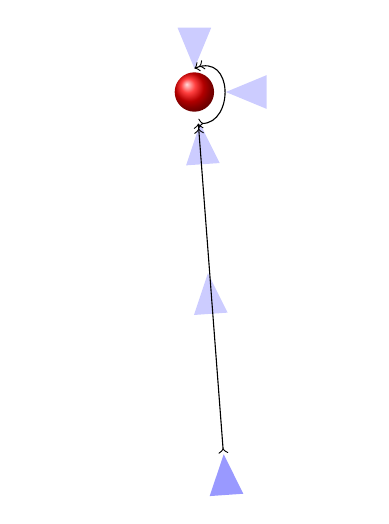
\begin{tikzpicture}
				\tikzstyle{ball} = [circle, shading=ball, ball color=red, minimum size=0.5cm]
				\node (ball) [style=ball] at (2.0,5.0) {};
				\node (botleft) at (0,0) {};
				\node (botright) at (4,0) {};
				\node (Nao0) at (2.4, 0) [isosceles triangle, fill=blue!40, rotate=94] {};
				\node (Nao1) at (2.2, 2.3) [isosceles triangle, fill=blue!20, rotate=94] {};
				\node (Nao2) at (2.1,4.2) [isosceles triangle, fill=blue!20, rotate=94] {};
				\node (Nao3) at (2.8,5.0) [isosceles triangle, fill=blue!20, rotate=180] {};
				\node (Nao4) at (2.0,5.7) [isosceles triangle, fill=blue!20, rotate=-90] {};
				\draw [>->>] (Nao0) -- (2.05,4.6);
				\draw [>->>] (2.05,4.6) .. controls (2.5,4.6) and (2.5,5.5) .. (2.0,5.3);
			\end{tikzpicture}
			\label{fig:linearapproach}
		}
		\quad
		\subfigure[The curve approach allows the robot to perform its angle rotation while walking towards the ball.]{
			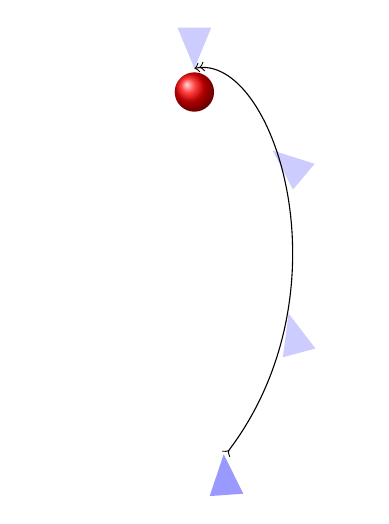
\begin{tikzpicture}
				\tikzstyle{ball} = [circle, shading=ball, ball color=red, minimum size=0.5cm]
				\node (ball) [style=ball] at (2.0,5.0) {};
				\node (botleft) at (0,0) {};
				\node (botright) at (4,0) {};
				\node (Nao0) at (2.4, 0) [isosceles triangle, fill=blue!40, rotate=94] {};
				\node (Nao1) at (3.3, 1.8) [isosceles triangle, fill=blue!20, rotate=105] {};
				\node (Nao2) at (3.3, 4.0) [isosceles triangle, fill=blue!20, rotate=140] {};
				\node (Nao3) at (2.0,5.7) [isosceles triangle, fill=blue!20, rotate=-90] {};
				\draw [>->>] (2.4,0.4) .. controls (4.0, 2.5) and (3.0, 5.5) .. (2.0,5.3);
			\end{tikzpicture}
			\label{fig:curveapproach}
		}
		\quad
		\caption{Difference between our original and our improved approach.}
	\end{figure}


\subsubsection{BodyFSM for the Goalie: Sagar}

\subsection{The Head Finite State Machine}
	The Head Finite State Machine (HeadFSM) controls the robot head movements. During the game, the robot has to move its head (changes yaw and pitch) efficiently to better and faster locate objects on field. The head movements are usually independent from the body movement, and therefore a separate state machine is designed. 

	Figure \ref{fig:headfsm} shows the HeadFSM (same for goalie and field players), followed by brief descriptions of the states. 
		
	\begin{figure}[H]
		\centering
		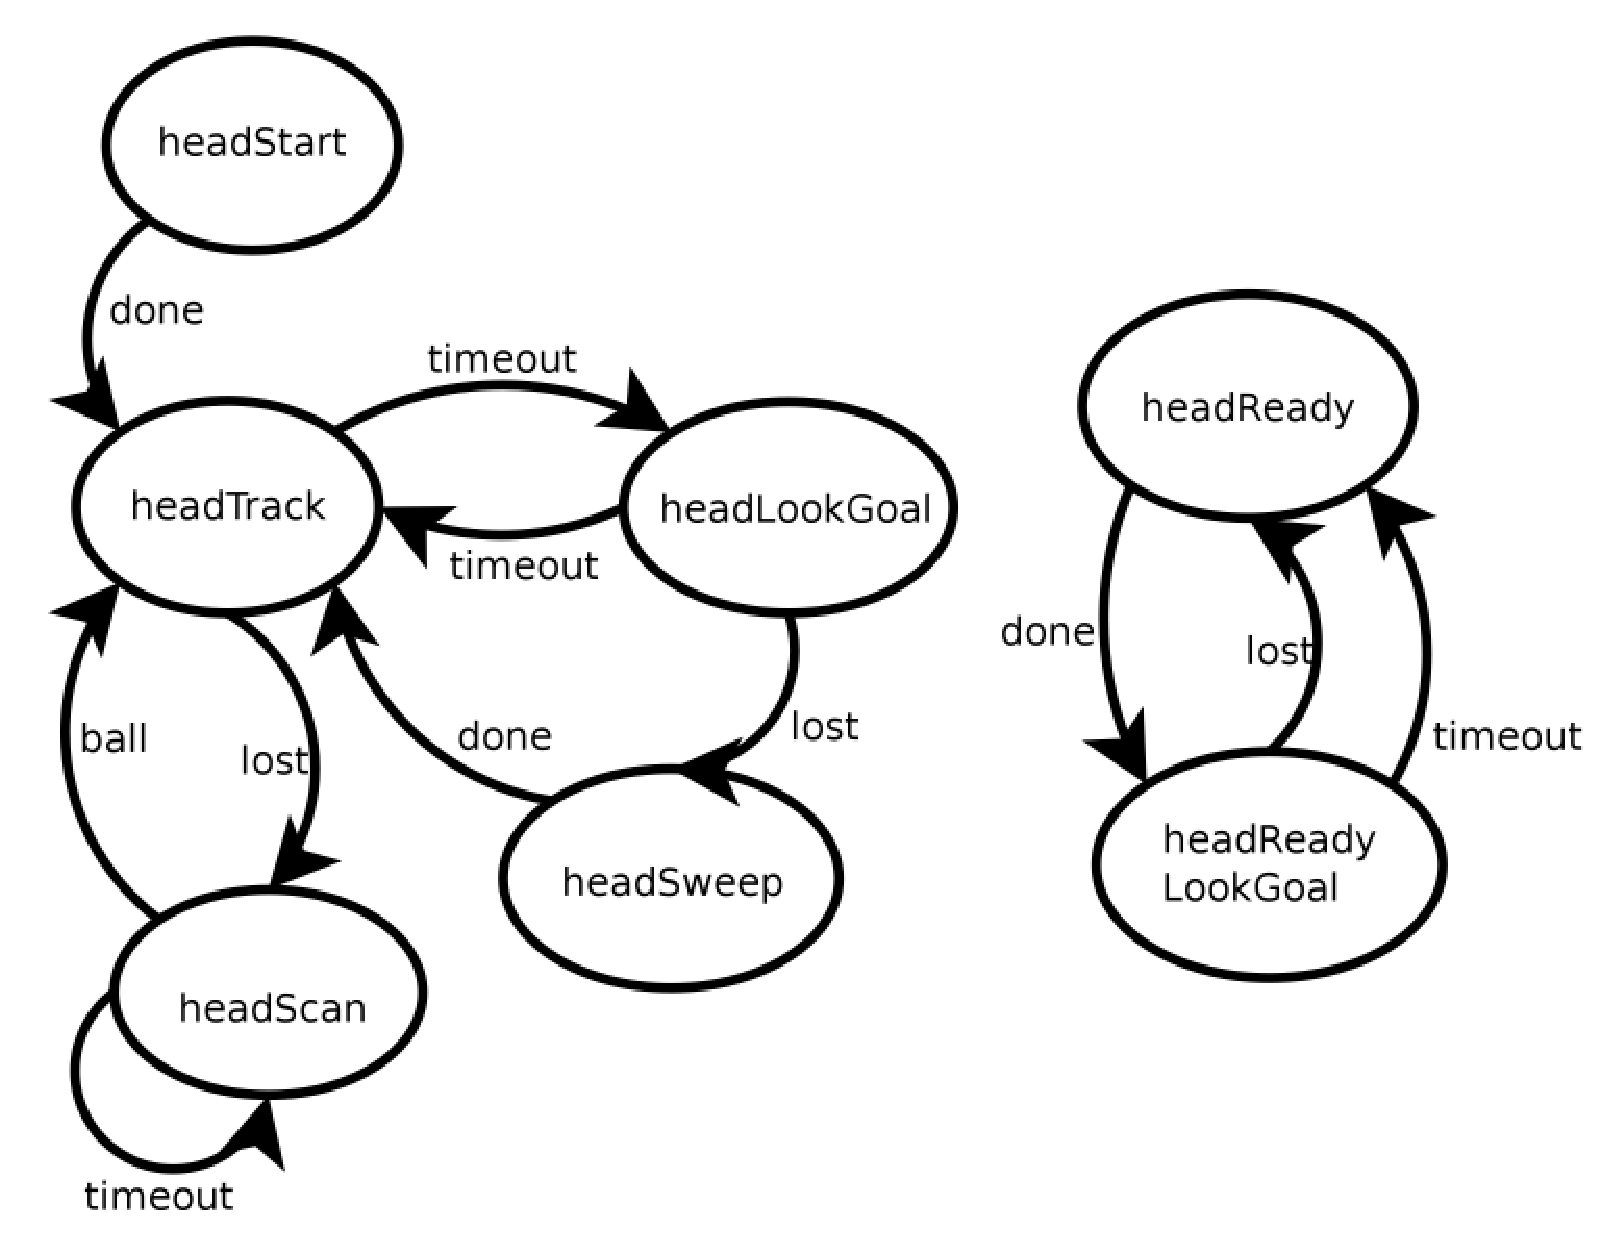
\includegraphics[width=.8\textwidth]{figures/HeadFSM.eps}
		\label{fig:headfsm}
		\caption{Head State Machine\\Left : during the game / Right: while waiting for game start }
		\label{fig:headfsm}
	\end{figure}

	\begin{multicols}{2}
		\begin{description}
			\item[headKick] During \textit{bodyApproach}, keep the head tilted down towards the ball.
			\item[headKickFollow] Follow the ball after a kick.
			\item[headLookGoal] Look up during approach to find the attacking goal posts.
			\item[headReady] Look for ball while waiting for game start
			\item[headReadyLookGoal] Look for goal while waiting for game start
			\item[headScan] Look around for the ball.
			\item[headStart] Initial state after the game state changes to 'Playing'.
			\item[headSweep] Perform a general search, with a priority on finding goal posts.
			\item[headTrack] Track the ball, moving or stationary.
		\end{description}
	\end{multicols}

\subsection{Team Play}
	Robust single robot behavior is not sufficient to have good performance during robot soccer games. All players on the field have to coordinate and function as a team. The team play module regulates team behaviors so robots can make efficient use of the space on field. The infrastructural base of team play is the WiFi-based communication between robots, where all players share basic cognition information (such as their own locations, the perceived ball locations, etc.) The essence of team play is a role switching mechanism which helps robots to stay at different locations on the field, contributing to both attacking and defending. There are five defined roles: 

	\begin{center}
		\begin{tabular}{ l c p{7cm} } %p{} takes care of text wrapping by defining a fixed column width.
			Goalie & 1 & Stays in and around the defensive goal to clear the ball when it comes close. \\
			Attacker & 2 & Goes directly towards the ball and kicks. \\
			Supporter & 3 & Follows the attacking robot up-field, but stays at a respectable distance away---usually about midfield. \\
			Defender & 4 & The defending robot positions itself between the ball and defensive goal area. \\					Defender Two & 5 & Performs double duty with the first defender, but has a different initial position. \\
		\end{tabular}
	\end{center}

	\begin{figure}[H]
		\centering
		\tikzstyle{ball} = [circle, shading=ball,ball color=red,minimum size=0.5cm]
		\subfigure[The ball is closest to Robot 2, the currently Attacker. Robot 3 sights the ball and is assigned Supporter.]{
		\begin{tikzpicture}
			\node (S) at (0, 0) [label=above:Supporter, isosceles triangle, fill=blue!30, text width=0.5cm, align=center, rotate=25] {\rotatebox{-25}{3}};
			\node (A) at +(40: 4.6) [label=left:Attacker, isosceles triangle, fill=blue!30, text width=0.5cm, align=center, rotate=-30] {\rotatebox{30}{2}};
			\node (E) at +(25: 7.0) [isosceles triangle, fill=red!30, text width=0.5cm, align=center, rotate=-150] {\rotatebox{150}{E}};
			\node (ball) [style=ball] at (4.9,2.2) {};
			\draw[->] (A) -- (ball);
			\draw[dotted, >->>] (S) -- (ball);
			\draw[dashed, o-)] (E) -- (ball);
		\end{tikzpicture}
		\label{fig:teamplay1}
		}
		\quad
		\subfigure[The opponent robot kicks the ball and the ball moves toward Robot 3, which becomes the new Attacker. The former Attacker Robot 2 is assigned Supporter due to further distance from the ball.]{
		\begin{tikzpicture}
			\node (S) at (0, 0) [label=above:Attacker, isosceles triangle, fill=blue!30, text width=0.5cm, align=center, rotate=5] {\rotatebox{-5}{3}};
			\node (A) at +(40: 4.6) [label=below:Supporter, isosceles triangle, fill=blue!30, text width=0.5cm, align=center, rotate=-118] {\rotatebox{118}{2}};
			\node (E) at +(25: 6.0) [isosceles triangle, fill=red!30, text width=0.5cm, align=center, rotate=-148] {\rotatebox{148}{E}};
			\node (ball) [style=ball] at (2.0,0.2) {};
			\draw[->] (S) -- (ball);
			\draw[dotted, >->>] (A) -- (ball);
			\draw[dashed, o-)] (E) -- (ball);
		\end{tikzpicture}
		\label{fig:teamplay2}
		}
		\quad
		\caption{Simple Example of Role Switching.}
	\end{figure}
	
	The primary strategy is to keep the ball moving down-field. To encourage this, the four general players (non-goalies) are constantly switching their roles. According to the shared cognition information, each robot calculates its estimated time of approaching (ETA). ETA is a function of numeral factors, including if the robot is fallen, if the robot sees the ball, the distance between the robot and the ball, walking speed, etc. The robot with the smallest ETA will be assigned the attacker, and other robots will be assigned defender or supporter based on their locations on field. Figure \ref{fig:teamplay1} and \ref{fig:teamplay2} is a illustration of dynamic role switching during the game.	


\section{Summary}
	While the UPennalizers broke their annual tradition of making it to the quarterfinal matches every year, the team has continued to keep pace with the rest of the league. With a new batch of undergraduates ready to pass on their knowledge to new team members in the fall, the UPennalizers' future looks as bright as ever.

\end{document}

